%Version 3 October 2023
% See section 11 of the User Manual for version history
%
%%%%%%%%%%%%%%%%%%%%%%%%%%%%%%%%%%%%%%%%%%%%%%%%%%%%%%%%%%%%%%%%%%%%%%
%%                                                                 %%
%% Please do not use \input{...} to include other tex files.       %%
%% Submit your LaTeX manuscript as one .tex document.              %%
%%                                                                 %%
%% All additional figures and files should be attached             %%
%% separately and not embedded in the \TeX\ document itself.       %%
%%                                                                 %%
%%%%%%%%%%%%%%%%%%%%%%%%%%%%%%%%%%%%%%%%%%%%%%%%%%%%%%%%%%%%%%%%%%%%%

%%\documentclass[referee,sn-basic]{sn-jnl}% referee option is meant for double line spacing

%%=======================================================%%
%% to print line numbers in the margin use lineno option %%
%%=======================================================%%

%%\documentclass[lineno,sn-basic]{sn-jnl}% Basic Springer Nature Reference Style/Chemistry Reference Style

%%======================================================%%
%% to compile with pdflatex/xelatex use pdflatex option %%
%%======================================================%%

%%\documentclass[pdflatex,sn-basic]{sn-jnl}% Basic Springer Nature Reference Style/Chemistry Reference Style


%%Note: the following reference styles support Namedate and Numbered referencing. By default the style follows the most common style. To switch between the options you can add or remove “Numbered” in the optional parenthesis. 
%%The option is available for: sn-basic.bst, sn-vancouver.bst, sn-chicago.bst%  
 
%%\documentclass[sn-nature]{sn-jnl}% Style for submissions to Nature Portfolio journals
%%\documentclass[sn-basic]{sn-jnl}% Basic Springer Nature Reference Style/Chemistry Reference Style
%%\documentclass[sn-mathphys-num]{sn-jnl}% Math and Physical Sciences Numbered Reference Style 
%%\documentclass[sn-mathphys-ay]{sn-jnl}% Math and Physical Sciences Author Year Reference Style
%%\documentclass[sn-aps]{sn-jnl}% American Physical Society (APS) Reference Style
%%\documentclass[sn-vancouver,Numbered]{sn-jnl}% Vancouver Reference Style
\documentclass[sn-apa]{sn-jnl}% APA Reference Style 
%%\documentclass[sn-chicago]{sn-jnl}% Chicago-based Humanities Reference Style

%%%% Standard Packages
%%<additional latex packages if required can be included here>

\usepackage{graphicx}%
\usepackage{multirow}%
\usepackage{amsmath,amssymb,amsfonts}%
\usepackage{amsthm}%
\usepackage{float}%
\restylefloat{table}
\usepackage{makecell}%
\usepackage{mathrsfs}%
\usepackage[title]{appendix}%
\usepackage{xcolor}%
\usepackage{textcomp}%
\usepackage{manyfoot}%
\usepackage{booktabs}%
\usepackage{algorithm}%
\usepackage{algorithmicx}%
\usepackage{algpseudocode}%
\usepackage{listings}%
%%%%

%%%%%=============================================================================%%%%
%%%%  Remarks: This template is provided to aid authors with the preparation
%%%%  of original research articles intended for submission to journals published 
%%%%  by Springer Nature. The guidance has been prepared in partnership with 
%%%%  production teams to conform to Springer Nature technical requirements. 
%%%%  Editorial and presentation requirements differ among journal portfolios and 
%%%%  research disciplines. You may find sections in this template are irrelevant 
%%%%  to your work and are empowered to omit any such section if allowed by the 
%%%%  journal you intend to submit to. The submission guidelines and policies 
%%%%  of the journal take precedence. A detailed User Manual is available in the 
%%%%  template package for technical guidance.
%%%%%=============================================================================%%%%

%% as per the requirement new theorem styles can be included as shown below
\theoremstyle{thmstyleone}%
\newtheorem{theorem}{Theorem}%  meant for continuous numbers
%%\newtheorem{theorem}{Theorem}[section]% meant for sectionwise numbers
%% optional argument [theorem] produces theorem numbering sequence instead of independent numbers for Proposition
\newtheorem{proposition}[theorem]{Proposition}% 
%%\newtheorem{proposition}{Proposition}% to get separate numbers for theorem and proposition etc.

\theoremstyle{thmstyletwo}%
\newtheorem{example}{Example}%
\newtheorem{remark}{Remark}%

\theoremstyle{thmstylethree}%
\newtheorem{definition}{Definition}%

\raggedbottom
%%\unnumbered% uncomment this for unnumbered level heads

\begin{document}

\title[Article Title]{Time Series Forecasting Using Recurrent Neural Networks Based on Recurrent Sigmoid Piecewise Linear Neurons }

%%=============================================================%%
%% GivenName	-> \fnm{Joergen W.}
%% Particle	-> \spfx{van der} -> surname prefix
%% FamilyName	-> \sur{Ploeg}
%% Suffix	-> \sfx{IV}
%% \author*[1,2]{\fnm{Joergen W.} \spfx{van der} \sur{Ploeg} 
%%  \sfx{IV}}\email{iauthor@gmail.com}
%%=============================================================%%

\author[1]{\fnm{Victor} \sur{Sineglazov}}\email{svm@nau.edu.ua}
\equalcont{These authors contributed equally to this work.}

\author*[1]{\fnm{Vladyslav} \sur{Horbatiuk}}\email{vladyslav.horbatiuk@npp.nau.edu.ua}

\affil*[1]{\orgdiv{Department of Aviation Computer Integrated Complexes}, \orgname{National Aviation University},
\orgaddress{\street{Liubomyra Huzara Ave 1}, \city{Kyiv}, \postcode{03058}, \country{Ukraine}}}


\abstract{We propose a new recurrent sigmoid piecewise linear neuron that can be used in neural networks to model time series when solving forecasting problem. The neuron is simpler than widely used long short-term memory and gated recurrent unit neurons and can be used as a drop-in replacement of these neurons. Simpler model of the new neuron results in faster training and inference of networks composed of such neurons. Besides theoretical analysis of the neuron's mathematical model the experiments on real world time series were performed to measure and compare accurracy of networks with different structures and used neuron types. Results of experiments show that networks with new neuron achieve similar or slightly better accuracy while having noticeably faster training and inference time.}

\keywords{recurrent neural networks, time series forecasting, sigmoid piecewise linear neuron, long short term memory neuron, gated recurrent unit neuron}

%%\pacs[JEL Classification]{D8, H51}

%%\pacs[MSC Classification]{35A01, 65L10, 65L12, 65L20, 65L70}

\maketitle

\section{Introduction}\label{sec1}

Forecasting is the process of predicting future events based on past and present data. Time series forecasting is a type of forecasting that predicts future events based on time-stamped data points. Time series forecasting models are an essential tool for any organization or individual who wants to make informed decisions based on future events or trends. From stock market forecasts to weather forecasts, time series models help us understand and predict changes over time. Forecasting is a part of statistical modeling that is widely used in various problems solutions and it is an important element of decision-making activity because whether an effective decision is made depends on forecasts accuracy. Nowadays, performing short-term and/or long-term and reliable time series forecasting remains as relevant as ever across a vast number of application domains, including healthcare \citep{kaushik2020ai}, meteorology \citep{faisal2022neural}, physiology \citep{ghassemi2015multivariate}, energy systems \citep{amasyali2018review}, econometrics \citep{sineglazov2018forecasting} amongst many others. 

Nowadays artificial neural networks are the most popular and widely used tool for many problems in areas like computer vision, natural language processing, autonomous driving and more. In the time series forecasting domain recurrent neural networks are often employed \citep{hewamalage2021recurrent} due to their suitability for sequential data processing and modelling. The popular choices for recurrent neurons to be used in neural networks are long short-term memory (LSTM) neuron \citep{hochreiter1997long} and gated recurrent unit (GRU) neuron \citep{cho2014learning} since these neurons are designed to better capture long-term dependencies in sequential data.

Recurrent networks composed of multiple layers of LSTM or GRU neurons are able to model pretty complex recurrent functions which is good when time series in question has a lot of available data points, but can be a disadvantage for smaller time series leading to overfittting and increased variance of predictions. Another practical drawback is relatively high training and inference speed of the model. In the paper we suggest a new recurrent sigmoid piecewise linear (RSPL) neuron which is based on sigmoid piecewise linear (SPL) neuron \citep{zgurovsky2018structural} and can be viewed as a simplified version of LSTM and GRU neurons (or just a GRU neuron, since it can also be considered a simplified version of LSTM neuron). As a result of RSPL neuron having a simpler model the networks composed of layers of this neuron are faster during both training and inference stages. Besides that, experiments on real time data have shown that replacing LSTM/GRU neurons in networks with RSPL neuron does not lead to decrease in accuracy on small time series.

The paper is organized as follows. An overview of related works is given in Sect. \ref{sec2}. Sect. \ref{sec3} gives a formal time series forecasting problem statement that is explored in this paper. Sect. \ref{sec4} presents a short overview of LSTM and GRU neurons. Sect. \ref{sec5} starts with an overview of SPL neuron and proceeds with introduction of RSPL neuron. Results of practical experiments on real world time series are given in Sect. \ref{sec6}.

The main contributions of this paper can be summarized as follows. This paper:
\begin{enumerate}
\item Proposes a new recurrent neuron - RSPL neuron - that may be used in layers of recurrent networks to model time series.
\item Explores the connection between RSPL, LSTM and GRU neurons.
\item Conducts practical experiments on real world time series to compare accuracy, training and inference speed of networks composed of layers of LSTM, GRU and RSPL neurons.  
\end{enumerate}

\section{Related works}\label{sec2}
There are many different types of time series forecasting models, each with their own strengths and weaknesses:

\begin{itemize}
\item ARIMA based models \citep{box2015time}.
\item Regression trees based models \citep{breiman2017classification}, including boosting trees approaches \citep{chen2016xgboost}.
\item Artificial intelligence models, notably approaches based on artificial neural networks (ANN) \citep{tealab2018time}.
\item Hybrid approaches, e.g. in \citep{fawzy2022comparative} authors use a combination of ANN and ARIMA models, in \citep{ngo2022developing} a combination of ARIMA and support vector regression \citep{awad2015support} is trained using firefly-inspired optimization algorithm \citep{fister2013comprehensive}, \citep{zaychenko2023investigation} uses ANN comprised of a neo-fuzzy neurons and GMDH-based \citep{ivakhnenko1995review} algorithm for simultaneous optimization of network structure and parameters.
\end{itemize}

\noindent
In recent years,  predicting financial time series utilizing Artificial Neural Network (ANN) applications has increased dramatically. The idea of ANN can be seen before reaching the output, where the filtration of the inputs through one or more hidden layers each of which consists of hidden units, or nodes is considered as the main idea. Thus, final output is related to the intermediate output [14]. The ability of learning from data through adaptive changing structure based on external or internal information that flows through the network during the learning phase and generates output variables based on learning is one of the most important advantages of ANN. Furthermore, the non-linear nature of ANN is also a valuable quality. ANNs are classified as non-linear data modeling tool, thus, one of the main purposes of utilizing such a model is to find the patterns in data or modeling complex relationships between inputs and outputs. Hence, an explicit model-based approach fails, but ANNs adapt irregularities and unusual of features in a time-series of interest. 

The application of ANNs has been popularly utilized in financial time series prediction modeling. However, as with many other techniques, ANNs have some disadvantages such as not allowing much of understanding of the data which might be because they are not explicit models. Therefore, providing a black box for the prediction process is considered as a disadvantage. The danger of over-fitting the in-sample training data is also a major ANN methods drawback [15]. In terms of the goodness of fit the performance of in-sample data sets is good, and is what ANNs are trained on. However, in out-of- ample data it is conditional on not breaking the structure in the data sets. According to Balestrassi et al. [16], excessive training time and large number of parameters that must be experimentally selected to obtain a good prediction are considered to be other disadvantages faced by ANN applications. 

Recurrent neural networks are well suited for supervised learning problems where the data set is sequential in nature. Time series forecasting should be no exception. RNNs are essentially neural networks with memory. They can remember events from the past, which is obviously useful for predicting time-dependent goals. 


\section{Time series forecasting problem}\label{sec3}
There are two different classes of time-series data: stationary and non-stationary data [x]. 

\begin{itemize}
\item Stationary time-series data is one where the statistical properties of the data do not change over time. In other words, the data does not exhibit any trend, seasonality, or other patterns that would cause these statistical properties to change. The random error is the only source of variability in the data set.
\item Non-stationary time-series data is a time-series data set that exhibits a trend or a seasonal effect. The random error is no longer the only source of variability in the data set. Non-stationary time-series data requires additional pre-processing, such as detrending or differencing, to remove the non-stationary before modeling and forecasting can be done accurately. 
\end{itemize}

\noindent
Time series forecasting problem considered in this paper can be stated as: there is a time series ${x_1, ..., x_N}$, generated by some probabilistic process $ \{X_t\} $ with unknown joint distributions: 
$$ p(x_{t+k}, x_{t}, x_{t-1}, ..., x_{t-n}). $$

The process $ \{X_t\} $ can be either stationary or non-stationary. If the process is non-stationary, in the general case this forecasting problem has no solution, since the probability distributions of a non-stationary series in theory can change "at will", and distributions in the future may have nothing in common with the distributions on the basis of which the existing time series was generated. However, in practice, changes in the probability distributions of non-stationary processes over time do not occur completely randomly. Therefore, predictive models evaluated on the available time series usually perform satisfactorily over a certain period of time, even if the corresponding process is non-stationary. 

It is necessary to use this time series to find a predictive model of the form:
$$ \hat{x}_{t+k} = f^*(x_{t}, ..., x_{t-n}), $$
which minimizes the mathematical expectation of the error: 
$$ f^* = argmin_f \{ E_{p(x_{t+k}, x_{t}, x_{t-1}, ..., x_{t-n})} [ L(f(x_{t}, ..., x_{t-n}), x_{t+k}) ] \}, $$
where:

\begin{itemize}
\item $L: \mathbb{R} \times \mathbb{R} \to \mathbb{R}_{\geq 0} $ - is the error function; often used is either quadratic $ L(x, \hat{x}) = (x-\hat{x})^2 $ or absolute error $ L(x, \hat{x}) = |x-\hat{x}| $
\item $k$ - forecasting horizon, i.e. how many steps ahead the forecast should be performed
\end{itemize}

\noindent
 Since it is impossible to calculate the real mathematical expectation (the corresponding probability distributions are unknown), the average value of the error function on the test subsample of the time series is used instead: 
 $$ f^* = argmin_f \{ \frac{1}{M} \sum_{t=N-k-M+1}^{N - k}{L(f(x_t, ..., x_{t-n}), x_{t+k})} \}, $$
where $M$ is a number of samples in the test subset.

We present the error metrics used to evaluate the predictions on the out-of-sample area of the data.  
To assess the forecast quality, the mean squared error (MSE) is a commonly used metric in comparing time series models. Its non-negativity as well as its symmetry are highly valuable features [x].
$$ MSE = \frac{1}{n}\sum_{i=1}^{n}{(X_i - Y_i)^2}, $$
where $X_i$ is the predicted target value at time step $i$, $Y_i$ is the true target value at time step $i$; $n$ is the quantity of predicted time steps. 
While the MSE has a symmetry, the root mean squared error (RMSE) $RMSE=\sqrt{MSE}$ evaluates larger errors stronger than smaller ones making it more sensitive to outliers and penalizing them [x]. This property must be kept in mind and can be beneficial as well as negative. Therefore, this metric is used in a context-specific manner. In the area of demand forecasting, it can be useful to use this metric to evaluate the models as well, since large errors in the forecast lead to major economic losses, for example in form of excessive inventory.  
Since both of the previously mentioned metrics are not scaled, it is difficult to compare the metrics from time series to time series and across multiple models. Kolossa and Siemsen [x] suggest for intermittent time series, to scale the RMSE by the series overall mean of the test set to obtain a scaled error measure that is comparable between time series. In the following we use the notation for this metric sRMSE:
$$ sRMSE = \frac{RMSE}{\frac{1}{n}\sum_{i}{Y_i}} $$
Symmetric Mean Absolute PercentageError (sMAPE) was originally used in the M3 Competition for evaluating the participating methods, is defined as follows: 
$$ sMAPE = \frac{1}{n}\sum_{i=1}^{n}{\frac{|X_i - Y_i|}{(|Y_i| + |X_i|)/2}} $$

\section{Recurrent Neural Networks with LSTM and GRU neurons }\label{sec4}
A recurrent neural network is a network where the connections between elements form a directed sequence. This makes it possible to process series of events in time or sequential spatial chains. Recurrent networks can use their internal memory to process sequences of arbitrary length. There are loops inside it, which implies the presence of short memory in the network. One of the issues of the recurrent neural network is related to sequence as a direct cycle is formed with their connections.  The  next state can be  retained using the current output as input for  the  next  step resembling  as  running  a  program  with  standard inputs  and  selected  internal  variables. 

RNNs are neural networks for sequential data - so they are applied to time series. The basic idea of recurrent neural networks is to use not only input data, but also previous output data to create a current forecast. However, they are difficult to train and forgetful. There are two popular and effective recurrent neural networks based on Long Short Term Memory (LSTM) \citep{hochreiter1997long} and gated recurrent unit (GRU) neurons \citep{cho2014learning}.
In natural language processing tasks, such as building language models, automatic text translation, etc., recurrent neural networks based on Long Short Term Memory (LSTM) and/or Gated Recurrent Unit (GRU) neurons have proven themselves well. These neurons have a similar structure that helps reduce the impact of the decaying/exploding gradient problem when training recurrent models using the Backpropagation Through Time (BPTT) algorithm on long sequences. 
The  default  behavior  LSTM  can capture  and  store  information  for  a  longer  span of time. The main component of LSTM is the cell state, a horizontal line that keeps running all through. The cell state always runs down the entire chain with less frequent interactions. It is very easy for information to just flow unchanged along with it. LSTM has all the rights to include or exclude the information to the cell  state,  that  are  let  through  by  structures  called gates.  It  is  a  way  to  decide  whether  to  let  the information through or not. It consists of a sigmoid network layer and performs multiplication operation. The  output  value  of  the  sigmoid  layer  ranges between  zero  and  one  indicating  the  individual component to decide whether to go through or not. A value zero indicates “let nothing through” and one indicates “let everything through”.   
Recurrent neural networks based on Long Short Term Memory (LSTM) and/or Gated Recurrent Unit (GRU) are more stable in training and have greater “accuracy” when working on long sequences. An LSTM neuron has the following structure: 

\begin{figure}[H]
\centering
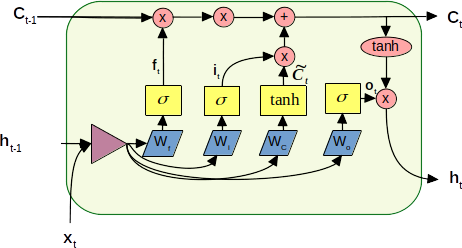
\includegraphics[width=0.6\textwidth]{lstm_neuron_structure.png}
\caption{LSTM neuron structure}\label{fig1}
\end{figure}
$$ f_t = \sigma( W_f \cdot [h_{t-1},x_t] + b_f) $$
$$ i_t = \sigma( W_i \cdot [h_{t-1},x_t] + b_i) $$
$$ \tilde{C_t} = tanh( W_C \cdot [h_{t-1},x_t] + b_C) $$
$$ C_t = f_t * C_{t-1} + i_t * \tilde{C_t} $$
$$ o_t = \sigma( W_o \cdot [h_{t-1},x_t] + b_o) $$
$$ h_t = o_t * tanh(c_t) $$

A GRU neuron is essentially a simplified version of an LSTM neuron: 
\begin{figure}[H]
\centering
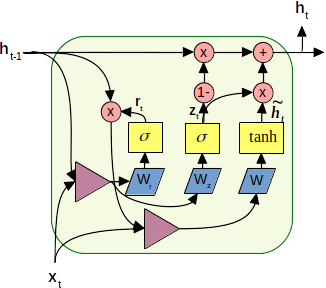
\includegraphics[width=0.45\textwidth]{gru_neuron_structure.png}
\caption{GRU neuron structure}\label{fig2}
\end{figure}
In this neuron, the output vector ht also performs the role of the context vector, and the following blocks are used:

\begin{itemize}
\item Update block $z_t(x_t,h_{t-1};W_z)$ that calculates weights in the range $(0, 1)$, which are used to calculate a new output vector (and, at the same time, context) $h_t$ based on the candidate vector $\tilde{h}_t$ and the previous vector $h_{t-1}$
\item Relevance block $r_t(x_t,h_{t-1};W_r)$ that calculates weights in the range $(0, 1)$ which determine the relevance of the values of the previous output vector $h_{t-1}$ when calculating the candidate vector for the new output vector $\tilde{h}_t$
\item Block for calculating the candidate vector of new outputs $\tilde{h}_t(x_t,h_{t-1},r_t;W)$
\item A block for calculating a new output vector $h_t(h_{t-1},\tilde{h}_t,z_t)$  as a weighted sum of the corresponding values from the previous vector $h_{t-1}$ and a new candidate vector $\tilde{h}_t$, where the weights for the values under index $i$ are chosen as $1-z_t[i]$ and $z_t[i]$ respectively. 
\end{itemize}

\section{Recurrent Sigmoid Piecewise Linear Neuron}\label{sec5}
This paper proposes a new model of a recurrent neuron, Recurrent Sigmoid. Piecewise (RSP), which is based on the Sigmoid Piecewise Linear (SPL) neuron \citep{zgurovsky2018structural}.
\subsection{The structure of the Sigmoid Piecewise neuron and its features}\label{subsec51}
Any continuous function $f: \mathbb{R}^n \to \mathbb{R} $ can always be approximated via a piecewise linear function that divides the space $\mathbb{R}^n$ into non-overlapping convex regions $S_1,S_2,...,S_N \in \mathbb{R}^n, S_i \cap S_j = \emptyset $  and defines a separate linear function for each region:
$$f_i(x) = w_i \cdot x, w_i \in \mathbb{R}^n.$$
Consider a simple piecewise linear neuron as a basic element for generating such complex piecewise linear functions:
\begin{equation}
  pl(x;w_+,w_-,h) =
    \begin{cases}
      w_+ \cdot x & \text{if $h \cdot x \ge 0$}\\
      w_- \cdot x & \text{if $h \cdot x < 0$}
    \end{cases}
    , w_+, w_-, h \in \mathbb{R}^n
\end{equation}
Parameters vectors $w_+,w_-,h$ have the following meaning: 
\begin{itemize}
\item $h \in \mathbb{R}^n$ defines a hyperplane that splits $\mathbb{R}^n$ in 2 halves
\item $w_+$ defines a linear function for the region where $h \cdot x \ge 0$
\item $w_-$ defines a linear function for the region where $h \cdot x < 0 $
\end{itemize}
The function $pl$ is obviously non-differentiable and not continuous at $x: h \cdot x = 0$. This issue can be resolved by using the following neuron model, called sigmoid piecewise linear (SPL) neuron:

$$ spl(x;w_+,w_-,h) = \frac{w_+ \cdot x}{1 + e^{-h \cdot x}} + \frac{w_- \cdot x}{1 + e^{h \cdot x}}, $$
If we rewrite piecewise linear neuron as:
$$ pl(x;w_+,w_-,h) = (w_+ \cdot x) \cdot \boldsymbol{1}_{[0;\infty)}(h \cdot x) + 
   (w_- \cdot x) \cdot \boldsymbol{1}_{(-\infty;0)}(h \cdot x) $$
we see that SPL neuron essentially approximates step functions $\boldsymbol{1}_{[0;\infty)}(h \cdot x)$ and $\boldsymbol{1}_{(-\infty;0)}(h \cdot x)$ using sigmoid functions $ \sigma_+(x;h) = \frac{1}{1 + e^{-h \cdot x}} $ and $ \sigma_-(x;h) = \frac{1}{1 + e^{h \cdot x}} $ respectively:

\begin{figure}[h]
\centering
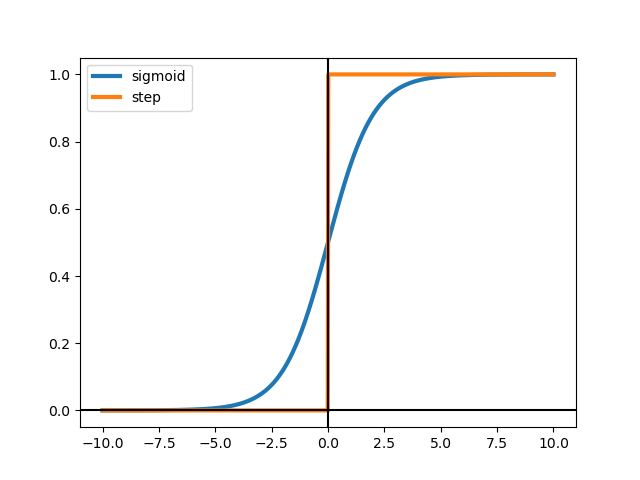
\includegraphics[width=0.7\textwidth]{step_vs_sigmoid.png}
\caption{Comparison of step and sigmoid functions}\label{fig2}
\end{figure}

Standard artificial neuron consists of two parts: a weighted adder $s(x;w) = w \cdot x$ and an activation function $a(y; \theta)$ (where $\theta$ is an optional vector of activation function's parameters), and the neuron itself is a composition of these parts:
$$f(x;w,\theta)=a(s(x;w);\theta)=a(w \cdot x; \theta)$$
In the case of SPL neuron the structure is somewhat more complicated: it consists of 3 weighted adders blocks $s_+(x;w_+),s_-(x;w_-),s_h(x;w_h)$ and an activation function of 3 variables:
$$a(s_+,s_-,s_h) = \frac{s_+}{1 + e^{-s_h}} + \frac{s_-}{1 + e^{s_h}},$$
that together compose "into" SPL neuron:
 $$spl(x;w_+,w_-,w_h) = a(s_+(x;w_+),s_-(x;w_-),s_h(x;w_h)).$$
 Unfortunately, because the SPL neuron's activation function is a function of three variables it is not  possible to plot it as a two- or three-dimensional graph. However, we can plot the graph with some additional constraints. For example, here is the three dimensional plot of the activation function with an added constraint $S_+=5S_-$:

\begin{figure}[H]
\centering
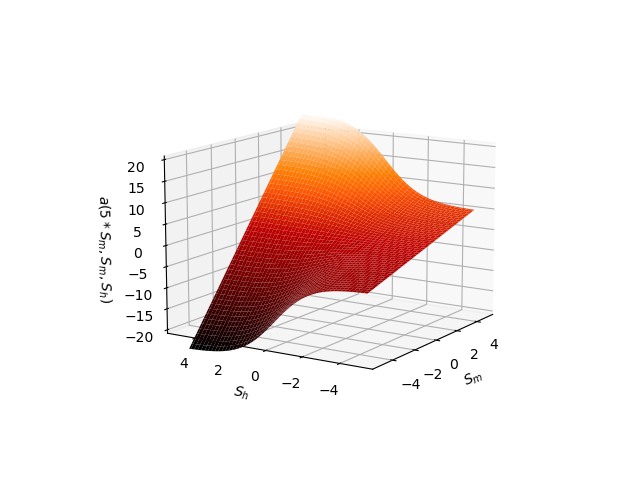
\includegraphics[width=0.7\textwidth]{spl_neuron_3d_plot_with_constraint_sp_eq_5sm.png}
\caption{3D plot of SPL neuron's activation function with added constraint $S_p=5S_m$}\label{fig2}
\end{figure}

In the context of building a predictive model for non-stationary time series with several potential conditional distributions, the Sigmoid Piecewise neuron can be considered as one of the simplest predictive models consisting of several local models and a component model that determines which of the local models to apply to a given input vector. That is, parameter vector $w_+$ specifies the first local model corresponding to one of the two potential distributions, vector $w_-$ – the second local model corresponding to the second potential distribution, and vector $h$ – the parameters of the component model that, according to the values of the input vector, determines which potential distribution is active - and therefore which local model to use to get the forecast. By combining several such neurons, it is already possible to simulate more than two potential conditional distributions. 
 
\subsection{Training the parameters of SPL neuron}\label{subsec52}
Since the mathematical model of the Sigmoid Piecewise neuron is a differentiable function of its parameters, their adjustment to minimize a certain function that depends on the output of the neuron can be performed using a certain modification of the gradient descent algorithm, using the following formulas for calculating the first derivatives:
$$\frac{\partial f}{\partial w_{+(q)}}=\frac{x_q}{1+e^{-h \cdot x}},$$
$$\frac{\partial f}{\partial w_{-(q)}}=\frac{x_q}{1+e^{h \cdot x}},$$
$$\frac{\partial f}{\partial h_q}=-\frac{w_+ \cdot x}{(1+e^{-h \cdot x})^2}e^{-h \cdot x}(-x_q)
-\frac{w_- \cdot x}{(1+e^{h \cdot x})^2}e^{h \cdot x}x_q=$$
$$=\frac{(w_+ \cdot x)x_q}{(1+e^{-h \cdot x})(1+e^{-h \cdot x})e^{h \cdot x}}-
\frac{(w_- \cdot x)x_q}{(1+e^{h \cdot x})(1+e^{h \cdot x})e^{-h \cdot x}}=$$
$$=\frac{(w_+ \cdot x)x_q}{(1+e^{-h \cdot x})(1+e^{h \cdot x})}-
\frac{(w_- \cdot x)x_q}{(1+e^{h \cdot x})(1+e^{-h \cdot x})}=$$
$$=\frac{(w_+ \cdot x)x_q - (w_- \cdot x)x_q}{(1+e^{-h \cdot x})(1+e^{h \cdot x})}=$$
$$=\frac{x_q(w_+ \cdot x - w_- \cdot x)}{2+e^{-h \cdot x} + e^{h \cdot x}}$$
So, we have the following 3D plots of the dependence of the values of the derivatives $\frac{\partial f}{\partial w_{+(q)}}$ and $\frac{\partial f}{\partial w_{-(q)}}$ on the values of $x_q$ and $s_h=h \cdot x$:

\begin{figure}[H]
\centering
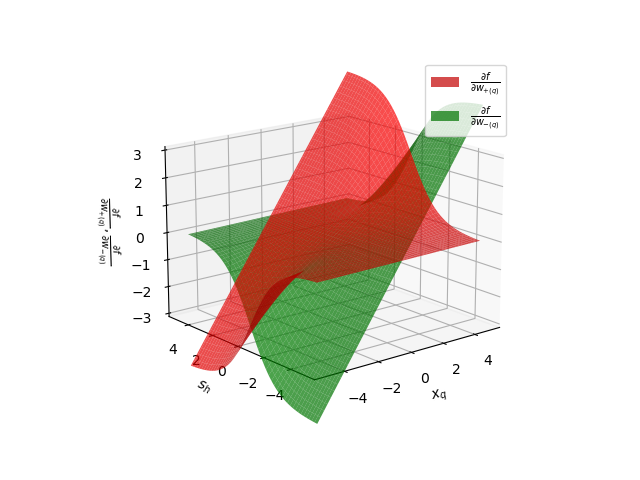
\includegraphics[width=0.7\textwidth]{spl_neuron_wp_wm_partial_derivatives_3d_surfaces.png}
\caption{3D plots of SPL neuron's partial derivatives w.r.t. $w_{+(q)}$ and $w_{-(q)}$}\label{fig3}
\end{figure}

And this is the plot of the dependence of the value of the derivative $\frac{\partial f}{\partial h_q}$ on the values $t=x_q(w_+ \cdot x - w_- \cdot x)$ and $s_h=h \cdot x$ looks like:

\begin{figure}[H]
\centering
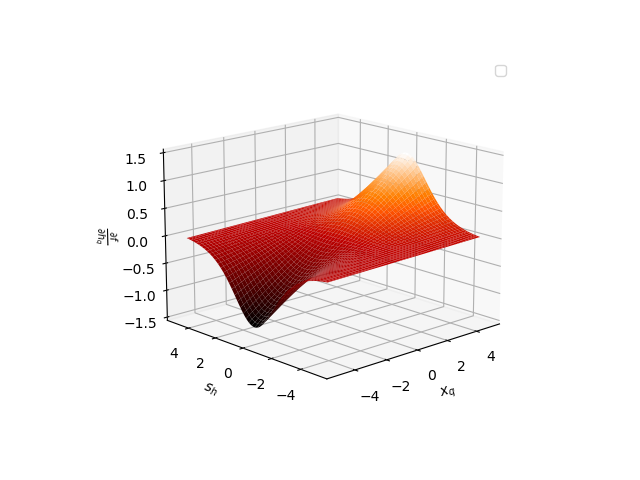
\includegraphics[width=0.7\textwidth]{spl_neuron_h_partial_derivative_3d_surface.png}
\caption{3D plot of SPL neuron's partial derivative w.r.t. $h_q$}\label{fig4}
\end{figure}

For further analysis of the "behavior" of the partial derivatives of the SPL neuron, it is also worth noting that the sum $\frac{\partial f}{\partial w_{+(q)}} + \frac{\partial f}{\partial w_{-(q)}}$ can be simplified as follows:
$$ \frac{\partial f}{\partial w_{+(q)}} + \frac{\partial f}{\partial w_{-(q)}} = 
	\frac{x_q}{1+e^{-h \cdot x}} + \frac{x_q}{1+e^{h \cdot x}} = $$
$$ \frac{x_q (1+e^{h \cdot x}) + x_q(1+e^{-h \cdot x})}{(1+e^{-h \cdot x})(1+e^{h \cdot x)}} =
	\frac{x_q (2+e^{h \cdot x}+e^{-h \cdot x})}{2+e^{h \cdot x}+e^{-h \cdot x}} = x_q$$
After analyzing these graphs and equations, the following conclusions can be drawn: 
\begin{enumerate}
\item The value $S_h=h \cdot x$ has an important influence on the value of all derivatives, that is, how far and on which side from the dividing plane specified by the vector $h$ is the input vector $x$.
\item Sum of derivatives $\frac{\partial f}{\partial w_{+(q)}} + \frac{\partial f}{\partial w_{-(q)}}$ is always equal to $x_q$. However, depending on the sign and the magnitude of $S_h$ the contribution of $\frac{\partial f}{\partial w_{+(q)}}$ and $\frac{\partial f}{\partial w_{-(q)}}$ will be different: if $S_h << 0$ - the value of $\frac{\partial f}{\partial w_{+(q)}}$ will be close to 0 and the value of $\frac{\partial f}{\partial w_{-(q)}}$ will be close to $x_q$, and vice versa when $S_h >> 0$. When $S_h \approx 0$ - contribution of both derivatives will be similar.
\item The derivative $\frac{\partial f}{\partial h_q} \approx 0 $ when $|S_h| >> 0 $ and $\approx \frac{x_q(w_+ \cdot x - w_- \cdot x)}{4}$ when $S_h \approx 0$. Thus, if the vector $x$ is far from the separating hyperplane defined by $h$ - it won't influence the training of vector $h$ very much. On the other hand, if $x$ is close to the hyperplane (i.e. $S_h \approx 0$) - the derivative $\frac{\partial f}{\partial h_q} $ will be proportional to $(w_+ \cdot x - w_- \cdot x)$. So the biggest influence on the correction of $h$ will be "caused" by inputs vectors $x$ such that: $h \cdot x \approx 0$ and $|w_+ \cdot x - w_- \cdot x| >> 0$. Besides that, if at some point during training all input vectors $x$ will have $h \cdot x >> 0$ - correction of $h$ will practically stop, since all derivatives $\frac{\partial f}{\partial h_q}$ will be close to 0. This can happen in two cases:
\begin{enumerate}
\item All input vectors are on 1 side of the separating hyperplane defined by $h$ - in this case SPL neuron will essentially be equivalent to the ordinary linear neuron, and only one of the vectors $w_+$ or $w_-$ will be tuned.
\item Some input vectors are on 1 side of the hyperplane and some are on another side, i.e. there are 2 clusters in input vectors which are linearly separable with a certain gap and we've found a corresponding "separation" hyperplane. In most practical cases this can be considered a good outcome, since we would probably want different linear models applied to different clusters of data. 
\end{enumerate}
\item If after some training step the vectors $w_+$ and $w_-$ become close - the derivative $\frac{\partial f}{\partial h_q}$ will be close to 0. However taking into account previous analysis items we can conclude that this situantion will not last too long unless all input vectors lie on the separating hyperplane defined by $h$.
\end{enumerate}
  
 To use the SPL neuron in multilayer neural networks, in addition to the derivative of the neuron function w.r.t. its parameters the derivative w.r.t. to the input variables $x_q$ is also required:
 \begin{align}
\frac{\partial f}{\partial x_q} &= \frac{h_q(w_+ \cdot x - w_- \cdot x)}
	{2+e^{-h \cdot x} + e^{h \cdot x}} + \frac{w_{+(q)}}{1 + e^{-h \cdot x}} +
	\frac{w_{-(q)}}{1 + e^{h \cdot x}} = \nonumber \\
&= \frac{\partial f}{\partial h_q}\frac{h_q}{x_q} + \frac{w_{+(q)}}{1 + e^{-h \cdot x}}
	+ \frac{w_{-(q)}}{1 + e^{h \cdot x}} \label{eqderivwrtinputs}
\end{align} 
 
 From the last equation, we can conclude that $\frac{\partial f}{\partial x_q}$ will be non-zero whenever $w_{+(q)} \ne 0 $ or $w_{_(q)} \ne 0$. 

\subsection{Recurrent SPL neuron and its features}\label{subsec53}
We propose a new recurrent neuron called Recurrent Sigmoid Piecewise Linear neuron (RSPL) which is based on the SPL neuron. So, we start at standard single SPL neuron:
$$ SP(x;w_+,w_-,s) = (1 - \sigma(x;s))(w_- \cdot x) + \sigma(x;s)(w_+ \cdot x) $$
Now, if we need to describe a layer of SPL neurons then vectors $w_+,w_-,s$ will be replaced by the matrices  $W_+,W_-,S$:
$$ SP(x;W_+,W_-, S) = (1 - \sigma(x;S)) * (W_- \cdot x) + \sigma(x;S) * (W_+ \cdot x) $$
By introducing the notation $ z = \sigma(x;S) $, $a = W_- \cdot x$  and $b = W_+ \cdot x$ we obtain:
$$ SP(x) = (1 - z) * a + z * b $$
Which is similar to the block for calculating the new output/state vector in the GRU/LSTM neuron: 
$$ h_t = (1-z_t)*h_{t-1} + z_t*\tilde{h}_t. $$
Thus, by slightly changing the SPL neuron, you can get its recurrent version, the RSPL neuron, which takes the vector $p_t=[h_{t-1}, x_t]$ as input and outputs $h_t$:
$$ h_t=RSP(p_t;W_c,S) = (1-\sigma(p_t;S))*p_t + \sigma(p_t;S)*(W_c \cdot p_t) $$
Or, by analogy with LSTM/GRU neurons, the mathematical model of an RSP neuron can be written in several stages/blocks:
$$ z_t = \sigma(S \cdot [h_{t-1}, x_t]) $$
$$ \tilde{h}_t = W_c \cdot [h_{t-1}, x_t] $$
$$ h_t = (1 - z_t) * h_{t-1} + z_t * \tilde{h}_t $$
\\
And present them in the form of a block diagram:
\begin{figure}[h]
\centering
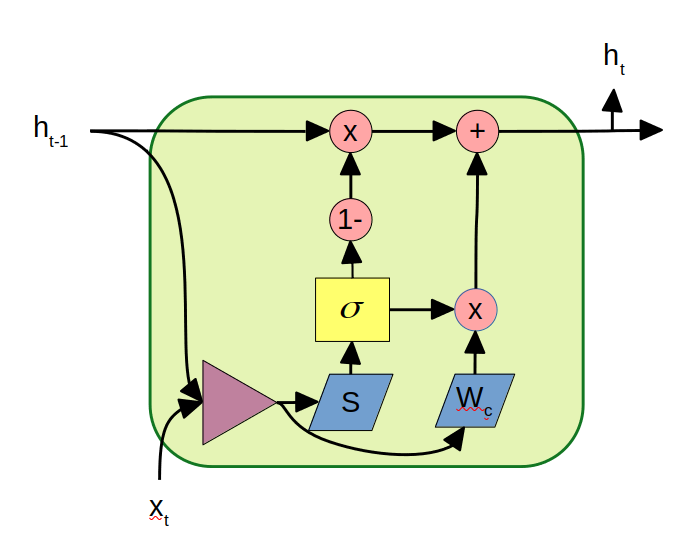
\includegraphics[width=0.5\textwidth]{recurrent_sigmoid_piecewise_neuron_structure.png}
\caption{GRU neuron structure}\label{fig3}
\end{figure}
\\
By superficially comparing the RSP neuron with LSTM and GRU neurons, the following observations can be made: 

\begin{itemize}
\item The mathematical model of the RSP neuron is simpler (only one nonlinear sigmoidal block is used) than the models of LSTM and GRU neurons. In the problem of time series forecasting, simpler models are often preferred in practice. 
\item At the same time, RSP, as well as LSTM and GRU neurons, allows you to forget certain values in the context vector if necessary. 
\end{itemize}

\section{RSPL neuron evaluation}\label{sec6}
To evaluate the effectiveness of using the RSP neuron in modeling the predicted time series, two real time series were used: 

\begin{itemize}
\item Daily values of the Dow Jones index for the period 2015/01/01-2023/1/1, total length of the time series - 2014 values:
\begin{figure}[h]
\centering
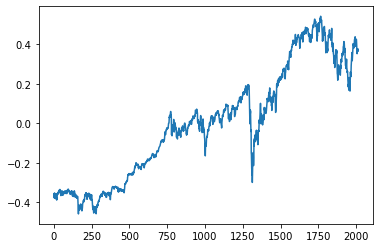
\includegraphics[width=0.5\textwidth]{dji_2015_01_01_2023_01_01.png}
\caption{GRU neuron structure}\label{fig4}
\end{figure}
\item OT (oil temperature) time series from the Electricity Transformer Dataset, which is often used to evaluate forecasting methods, with a total time series length of 5000 values \citep{haoyietal-informer-2021}:
\begin{figure}[h]
\centering
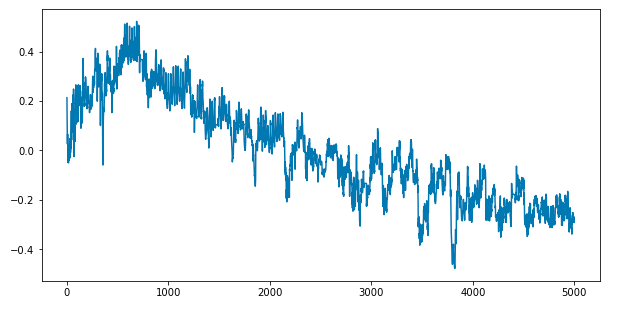
\includegraphics[width=0.5\textwidth]{etth_ot_time_series.png}
\caption{GRU neuron structure}\label{fig5}
\end{figure}

\end{itemize}

These series were divided into training and test sets, after which the model parameters were adjusted on the training set and metrics were calculated on the test set. To bring the original time series to a “more stationary form,” an optimal linear predictor was first selected for each training sample, after which the corresponding recurrent network was “set” with the task of predicting the deviation of the real value of the time series from the forecast of the linear predictor. Two previous values of the time series were used as input to the network to predict the next value; the learning rate for all models was set to 0.001, maximum number of training epochs to 300. To compare RSP neuron with LSTM and GRU in various network configurations, the following values of hyperparameters were tested: number of network layers $\in [1, 3, 5]$, dimension of the hidden state vector $\in [4, 8, 32]$.
In total, given 3 choices for the neuron type, 3 choices for the number of layers, and 3 choices for the dimension of the hidden state vector, 27 different models were trained for each time series. For each model, the error values on the test set were calculated once every 20 training epochs, and the time spent on completing each epoch was also logged. Summary of the obtained results: 
\\
\begin{table}[H]
\caption{Results summary for different network configurations on the Dow Jones index time series}
\begin{tabular}{|p{1.4cm}|p{1.4cm}|p{1.4cm}|p{1.5cm}|p{2.5cm}|p{1.9cm}|p{2cm}|}
\hline
Number of layers & Hidden layer size & Neuron type & Best test error & Relative best test error & Mean epoch time (s) & Relative mean epoch time\\
\hline
 1 &   4 &   RSP & 0.0065 & 1.0427 & 0.5714 &  1.0000 \\
\hline
 1 &   4 &   GRU & 0.0080 & 1.2818 & 0.6393 &  1.1187 \\
\hline
 1 &   4 &  LSTM & 0.0062 & 1.0000 & 0.7121 &  1.2461 \\
\hline
 1 &   8 &   RSP & 0.0063 & 1.0236 & 0.5749 &  1.0000 \\
\hline
 1 &   8 &   GRU & 0.0063 & 1.0176 & 0.6477 &  1.1266 \\
\hline
 1 &   8 &  LSTM & 0.0062 & 1.0000 & 0.7148 &  1.2434 \\
\hline
 1 &  32 &   RSP & 0.0062 & 1.0000 & 0.5790 &  1.0000 \\
\hline
 1 &  32 &   GRU & 0.0062 & 1.0001 & 0.6602 &  1.1404 \\
\hline
 1 &  32 &  LSTM & 0.0063 & 1.0128 & 0.7805 &  1.3482 \\
\hline
 3 &   4 &   RSP & 0.0068 & 1.0794 & 1.3176 &  1.0000 \\
\hline
 3 &   4 &   GRU & 0.0063 & 1.0000 & 1.5118 &  1.1475 \\
\hline
 3 &   4 &  LSTM & 0.0067 & 1.0753 & 1.8286 &  1.3879 \\
\hline
 3 &   8 &   RSP & 0.0067 & 1.0796 & 1.3112 &  1.0000 \\
\hline
 3 &   8 &   GRU & 0.0063 & 1.0292 & 1.5177 &  1.1575 \\
\hline
 3 &   8 &  LSTM & 0.0062 & 1.0000 & 1.8187 &  1.3870 \\
\hline
 3 &  32 &   RSP & 0.0062 & 1.0097 & 1.3277 &  1.0000 \\
\hline
 3 &  32 &   GRU & 0.0062 & 1.0041 & 1.5323 &  1.1541 \\
\hline
 3 &  32 &  LSTM & 0.0061 & 1.0000 & 1.9881 &  1.4975 \\
\hline
 5 &   4 &   RSP & 0.0063 & 1.0179 & 2.0749 &  1.0000 \\
\hline
 5 &   4 &   GRU & 0.0069 & 1.0998 & 2.4140 &  1.1635 \\
\hline
 5 &   4 &  LSTM & 0.0062 & 1.0000 & 2.9418 &  1.4178 \\
\hline
 5 &   8 &   RSP & 0.0065 & 1.0263 & 2.0498 &  1.0000 \\
\hline
 5 &   8 &   GRU & 0.0063 & 1.0000 & 2.4031 &  1.1724 \\
\hline
 5 &   8 &  LSTM & 0.0071 & 1.1170 & 2.9154 &  1.4223 \\
\hline
 5 &  32 &   RSP & 0.0065 & 1.0409 & 2.0939 &  1.0000 \\
\hline
 5 &  32 &   GRU & 0.0062 & 1.0067 & 2.4391 &  1.1649 \\
\hline
 5 &  32 &  LSTM & 0.0062 & 1.0000 & 3.1976 &  1.5271 \\
\hline
\end{tabular}
\end{table}

\begin{table}[H]
\caption{Results summary for different network configurations on the OT ETTH time series}
\begin{tabular}{|p{1.4cm}|p{1.4cm}|p{1.4cm}|p{1.5cm}|p{2.5cm}|p{1.9cm}|p{2cm}|}
\hline
Number of layers & Hidden layer size & Neuron type & Best test error & Relative best test error & Mean epoch time (s) & Relative mean epoch time \\
\hline
1 &   4 &   RSP & 0.0030 & 1.0030 & 1.4462 &  1.0000 \\
\hline
1 &   4 &   GRU & 0.0030 & 1.0000 & 1.6299 &  1.1270 \\
\hline
1 &   4 &  LSTM & 0.0031 & 1.0334 & 1.8409 &  1.2729 \\
\hline
1 &   8 &   RSP & 0.0030 & 1.0000 & 1.4436 &  1.0000 \\
\hline
1 &   8 &   GRU & 0.0030 & 1.0240 & 1.6246 &  1.1254 \\
\hline
1 &   8 &  LSTM & 0.0030 & 1.0021 & 1.8294 &  1.2672 \\
\hline
1 &  32 &   RSP & 0.0029 & 1.0000 & 1.4709 &  1.0000 \\
\hline
1 &  32 &   GRU & 0.0030 & 1.0072 & 1.6553 &  1.1254 \\
\hline
1 &  32 &  LSTM & 0.0030 & 1.0164 & 1.9888 &  1.3521 \\
\hline
3 &   4 &   RSP & 0.0031 & 1.0129 & 3.3214 &  1.0000 \\
\hline
3 &   4 &   GRU & 0.0031 & 1.0000 & 3.9134 &  1.1782 \\
\hline
3 &   4 &  LSTM & 0.0032 & 1.0281 & 4.6709 &  1.4063 \\
\hline
3 &   8 &   RSP & 0.0031 & 1.0181 & 3.2960 &  1.0000 \\
\hline
3 &   8 &   GRU & 0.0030 & 1.0014 & 3.9221 &  1.1899 \\
\hline
3 &   8 &  LSTM & 0.0030 & 1.0000 & 4.6470 &  1.4099 \\
\hline
3 &  32 &   RSP & 0.0030 & 1.0225 & 3.3440 &  1.0000 \\
\hline
3 &  32 &   GRU & 0.0029 & 1.0000 & 3.9690 &  1.1869 \\
\hline
3 &  32 &  LSTM & 0.0030 & 1.0269 & 5.0812 &  1.5195 \\
\hline
5 &   4 &   RSP & 0.0030 & 1.0000 & 5.2663 &  1.0000 \\
\hline
5 &   4 &   GRU & 0.0031 & 1.0200 & 6.1705 &  1.1717 \\
\hline
5 &   4 &  LSTM & 0.0032 & 1.0841 & 7.6743 &  1.4573 \\
\hline
5 &   8 &   RSP & 0.0030 & 1.0000 & 5.2238 &  1.0000 \\
\hline
5 &   8 &   GRU & 0.0031 & 1.0413 & 6.1681 &  1.1808 \\
\hline
5 &   8 &  LSTM & 0.0031 & 1.0230 & 7.6274 &  1.4601 \\
\hline
5 &  32 &   RSP & 0.0030 & 1.0098 & 5.3234 &  1.0000 \\
\hline
5 &  32 &   GRU & 0.0030 & 1.0198 & 6.2275 &  1.1698 \\
\hline
5 &  32 &  LSTM & 0.0029 & 1.0000 & 8.3525 &  1.5690 \\
\hline
\end{tabular}
\end{table}

In these tables, "relative best test error" and "relative mean epoch time" were calculated by dividing the corresponding absolute value by the minimum value among all 3 neuron types for the given hyperparameters configuration. That is, for each specific configuration of the number of layers and the hidden layer size there are 3 rows, one for each type of neuron; among these 3 rows, the row for the neuron with the smallest absolute best test error will have a relative best test error value equal to 1, and all others will have some values >= 1, similarly for the absolute and relative mean epoch time. 

If we average the relative parameters for each neuron over all possible configurations, we obtain the following results: 

\begin{table}[H]
\caption{Aggregated results on the Dow Jones index time series}
\begin{tabular}{ |p{2.2cm}|p{5cm}|p{5cm}| }
 \hline
  Neuron type & Aggregated relative best test error & Aggregated relative mean epoch time \\
  \hline
 RSP & 1.03556 & 1.0 \\
 \hline  
 GRU & 1.0488 & 1.1495 \\
 \hline 
 LSTM & 1.0228 & 1.38636 \\
 \hline
\end{tabular}
\end{table}

\begin{table}[H]
\caption{Aggregated results on the ET OTTH time series}
\begin{tabular}{ |p{2.2cm}|p{5cm}|p{5cm}|  }
 \hline
  Neuron type & Aggregated relative best test error & Aggregated relative mean epoch time \\
  \hline
 RSP & 1.00736 & 1.0 \\
 \hline  
 GRU & 1.01264 & 1.16169 \\
 \hline 
 LSTM & 1.02377 & 1.4127 \\
 \hline
\end{tabular}
\end{table}

\begin{table}[H]
\caption{Aggregated results for both time series}
\begin{tabular}{ |p{2.2cm}|p{5cm}|p{5cm}|  }
 \hline
  Neuron type & Aggregated relative best test error & Aggregated relative mean epoch time \\
  \hline
 RSP & 1.02146 & 1.0 \\
 \hline  
 GRU & 1.030724 & 1.1556 \\
 \hline 
 LSTM & 1.02328 & 1.3995 \\
 \hline
\end{tabular}
\end{table}

Overall summary regarding RSP neuron: 

• for the DJI series, the relative best test error averaged over all configurations ranks 2nd after LSTM 

• for the OT ETTH series - 1 place 

• relative time per epoch, averaged over all configurations for both series is 1.0, which is approximately 15.5% faster than the next “fastest” neuron – GRU 

• if we average the relative best test error over all configurations and over both time series, RSP takes 1st place. 

To compare pure inference speed of the RSP neuron we measure the average computation time of networks with GRU and RSP neurons among 100,000 runs for different values of the input vector size and hidden layer size. The LSTM neuron, as is known from the literature, is generally slower than the GRU.

\begin{table}[H]
\caption{Average computation time of networks with GRU/RSP neurons and different configurations}
\begin{tabular}{ |p{2cm}|p{2cm}|p{2cm}|p{2cm}|p{2cm}|p{2cm}|  }
 \hline
  Input and hidden layer size & 8, 64 & 4, 12 &  4, 32 & 2, 8 & 2, 16 \\
  \hline
 GRU & 0.054 ms & 0.0487 ms & 0.0503 ms & 0.0492 ms & 0.0507 ms \\
 \hline 
 RSP & 0.0355 ms & 0.032 ms & 0.0327 ms & 0.0317 ms & 0.032 ms \\
 \hline
\end{tabular}
\end{table}

As can be seen from the table, networks with RSP neuron are on average 1.58 times faster than networks of the same structure with GRU neuron.

\section{Conclusion}\label{sec7}
In this paper, we have presented a new recurrent neuron - RSPL, that could be used in neural networks for modelling time series forecasting. It is based on the sigmoid piecewise linear neuron and can be viewed as a simplified version of a well known GRU recurrent neuron. RSPL neuron could be used as a drop-in replacement in any networks that use LSTM or GRU neurons.
\\
Real-world data analyses on multiple time series and multiple neural network configurations have shown that networks with RSPL neurons achieve similar or better accuracy on test when compared with networks that use LSTM or GRU neurons. At the same time, training and inference speed for networks with RSPL neurons is noticeably faster.
\\ 
We acknowledge that the subsampling strategy based on K-means clustering may make
the results less interpretable. In the future, we aim to explore alternative sampling strategies
to enhance the interpretability of the results. For instance, in the univariate scenario, instead
of relying solely on K-means clustering, we can consider modifying the encoding process
by applying quantile thresholds to identify extreme observations, as discussed in Wang and
Hsieh (2022). Moreover, we plan to investigate other encoding techniques that are more
tailored to specific data characteristics. For multivariate data, alternative clustering algorithms or dimensionality reduction techniques may be explored to improve the efficiency
and interpretability of the encoding process.


\bibliography{paper}% common bib file

\end{document}
